\documentclass[12pt]{article}
\usepackage[utf8]{inputenc}

\usepackage[symbol]{footmisc} % footnote symbols

\usepackage{graphicx}
\graphicspath{ {output/} } % compile mode must be normal for images to display

\usepackage[
    letterpaper, 
    portrait, 
    margin=1in]{geometry} % set paper size, orientation, and margins
    
\usepackage[
    backend=biber,
    style=apa]{biblatex} % Imports biblatex package
    
\addbibresource{ref.bib} % Import the bibliography file

% set line spacing
\setlength{\parindent}{3em}
\setlength{\parskip}{0em}
\renewcommand{\baselinestretch}{1.5}

\renewcommand{\thefootnote}{\fnsymbol{footnote}}




\begin{document}

\hspace{5pt}

\Large
 \begin{center}
High Resolution Estimates of Agricultural Land Valuation for Conservation Efforts\footnote[2]{Acknowledgements go here.}\\ 

\vspace{10pt}

% Authors
\large
Asa Gold$^1$, Seth Binder$^2$, Christoph Nolte$^3$ \\

\vspace{10pt}

\footnotesize  
$^{1,2}$St. Olaf College\\
$^3$Boston University

\vspace{40pt} 

    \normalsize
    \textbf{Abstract}
\end{center}

\small
Conservation efforts, facing a fundamental scarcity of available resources and a wide array of potential conservation strategies, have suffered when informed by poor estimates of land value.

\newpage

Agencies designing conservation efforts must contend with the fundamental scarcity of available resources, while simultaneously confronting a vast array of potential conservation strategies. Accurately predicting costs of competing methods, then, is crucial to the efficient use of scarce conservation dollars. Such efficient use, however, is often impeded the poor quality of predictions at regulators' disposal concerning the fair market value of the underlying land. As recent work has demonstrated, previous efforts to predict fair market value have systematically and substantially underestimated costs of conservation (\cite{Nolte2020High-resolutionStates}). Particularly problematic has been farmland, a primary target for conservation advocates, either as a bulwark against further development or to recover natural ecosystems from degrading agricultural practices, such as monocropping. But because farmland value does not exhibit dynamics identical to those of other land types, appraisals that do not address agricultural property as a unique entity will fail to accurately portray the costs of bringing farmland under the aegis of regulatory agencies or non-profits like the Nature Conservancy. In Nolte (2020)'s analysis, the massive scope does not treat the drivers of agricultural land value as distant from other land types.

\par To fill this gap, we estimate fair market value of agricultural parcels nationwide. Building on a vast literature of Ricardian climatological impacts on agricultural valuation, as well as more recent attempts to estimate fair market value of parcels using machine learning methods trained on big data, we construct a rich parcel-level dataset to produce novel predictions of agricultural land value. Expanding Nolte (2020)'s work, we add variables on soil type, irrigation, and climatic conditions, and employ three distinct modeling strategies (linear regression, AIC ----FINALIZE----, and random forest) at three geographic levels (county, farm resource region, and national). In focusing solely on agricultural land, we are able to more fully capture the particular drivers of land valuation in agriculture-specific markets, contributing to more informed private and public decision making  stakeholders working to protect crucial ecosystems require increasingly accurate cost estimates when weighing competing strategies.

BRIEF DESCRIPTION OF FINDINGS

\section{Background}
Beginning in the 1990s, environmental and land economics has developed a rich literature under the broad class of Ricardian land value estimation, in which traditional econometric models are fit to data on observed sale price and climate conditions to unveil how physical features of a property are capitalized into its market value. Since (\cite{Mendelsohn1994TheAnalysis}), the literature has expanded into a variety of subfields, most notably studies on how agricultural value and productivity respond to climatic changes (\cite{Schlenker2005WillApproach}; \cite{Schlenker2006TheConditions}; \cite{Nelson2014ClimateShocks}; \cite{Mendelsohn2003ClimateAgriculture}; \cite{Bozzola2018AAgriculture}). More recent work has produced evidence of highly nonlinear relationships between, for instance, agricultural yields--a core factor in valuation--and anthropogenic climate change (\cite{Schlenker2006NonlinearYields}; \cite{Schlenker2009NonlinearChange}), suggesting modeling approaches should move beyond mere linear panel regression techniques traditionally used in the literature.

\par Today, a more empirical approach grounded in machine learning and data science has emerged, using a diverse array of cost proxies to estimate some variation of land value nationwide (\cite{Withey2012MaximisingUSA}; 
\cite{Johnson2020AReduction}; \cite{Lawler2020PlanningConfiguration}), with Nolte (2020) marking the most recent and, to our knowledge, most accurate and validated effort. The high resolution and massive scale (N = 6.01 million) of Nolte's data, enabled in aprt by Zillow's limited-offer ZTRAX repository, allows for parcel-specific analysis down to fractions of a hectare (\cite{Zillow2019ZTRAX:2019-Q4}). For comparison, the USDA's National Agricultural Statistics Service land value estimates operate at a resolution of around one square mile (\cite{USDepartmentofAgriculture2019AgriculturalEstimates}). Nolte's models employ variables on location, built environment, local demographics, and physical landscape features. To integrate Nolte (2020) with the broader Ricardian literature, we add further climatic and physical variables based on their use in Ricardian studies. In addition, we expand the modeling approach, using both a tree-based bagging algorithm and linear regression at three geographic scales.

\section{Data and Methods}
We base our analysis on data first published by Nolte (2020), a comprehensive high-resolution dataset of parcel characteristics and sales across the contiguous United States (140.9 million properties across 3,055 counties), including variables on building presence, development, accessibility, local demographics, local nature preservation, terrain, water, flood risk, land cover type, location, and date of sale. To these base data, we add several more variables aimed at improving the predictive accuracy of the fair market value models.


Soil classifications, indicating a map unit's suitability for agricultural use, were compiled from the Natural Resources Conservation Service’s high-resolution SSURGO soil survey database (\cite{SoilSurveyStaffSoilStates}). Soil classifications are operationalized as the percent of each parcel containing a given classification (e.g., “Prime Farmland” or “Farmland of Statewide Importance”). Aggregation is applied to overlapping classifications containing multiple conditions. For instance, "Prime if drained or protected from flooding" gets assigned to "Prime if drained" and Prime if protected from flooding." Climate normals of minimum, mean, and maximum monthly precipitation, temperature, and dew temperature were collected from \textbf{SOURCE} and aggregated by meterological season. Irrigation, soil, and climate variable coverage extends across the conterminous United States.  \textbf{LANID DESCRIPTION} \cite{Xie2021LANID-US:States}. Two new binary irrigation variables are created to record 1) whether the parcel had ever been irrigated prior to sale, and 2) whether it was irrigated at any point in the 3 years immediately preceding the sale. In the case of multi-parcel sales, we aggregate features across parcels (see Appendix).

With this expanded dataset, we model the fair market value of parcels in two ways: linear regression and extremely randomized trees, a decision tree-based bagging algorithm. Observed sale price is used as the conservation cost proxy in both modeling scenarios, which compare based on predictive accuracy, explanatory power, and variable importance or significance. Following Nolte (2020), the analysis is parallelized at the county level. We specify further models at the farm resource region level. Each linear regression exists in two forms: a baseline model including all 27 variables in Nolte (2020)’s analysis, as well as our added climate, soil, and irrigation variables; and a parsimonious model selected using Akaike information criterion. Extremely randomized trees are built with 500 base learners (trees), $\frac{p}{3}$ random features tried at each split, where $p$ is the total set of predictive features, and a required minimum leaf size of 3.

As our outcome variable, we use logged per-hectare price, adjusted by monthly consumer price index values for all urban consumers with a base year of 2020, using 5 million unique sales nationwide. In the case of county-level modeling, counties with under 1000 observations are augmented with randomly sampled sales from neighboring counties until they reach 1000 observations. If the county and its neighbors combined fail to achieve 1000 observations, no model is specified. 

\newpage

\section{Results}

RESULTS

\begin{figure}
    \centering
    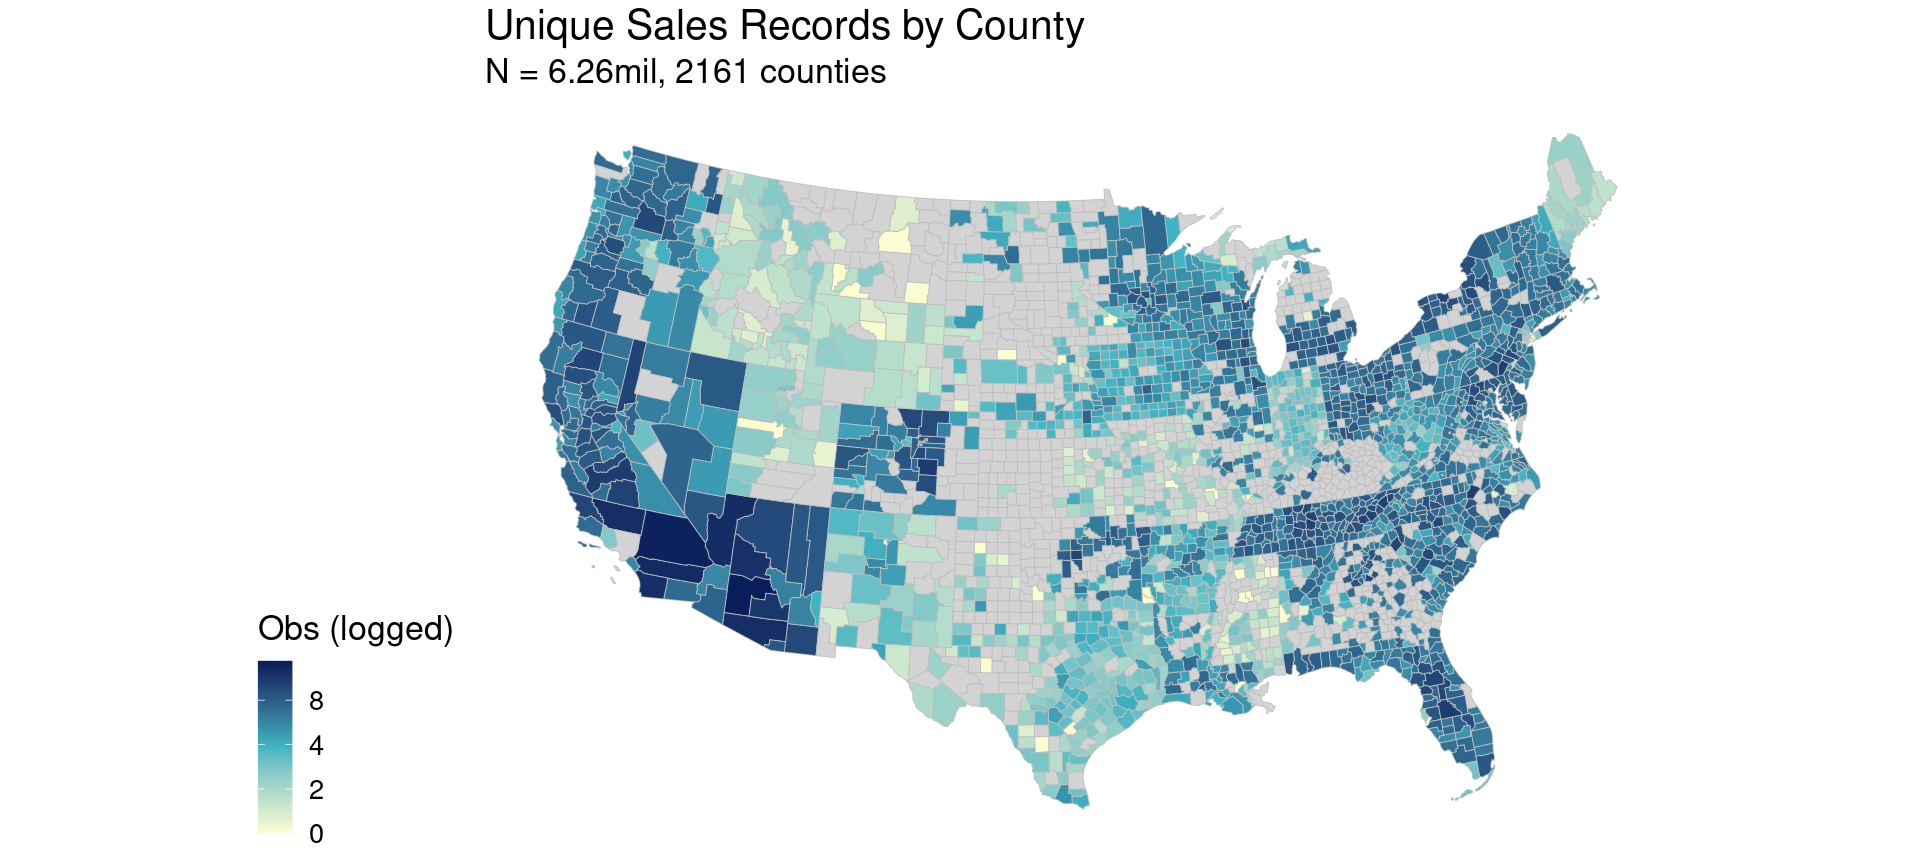
\includegraphics[width=6in]{eda_images/countysales_log.png}
    \caption{Sales By County}
    \label{fig:sales_county}
\end{figure}

More text.

\begin{figure}
    \centering
    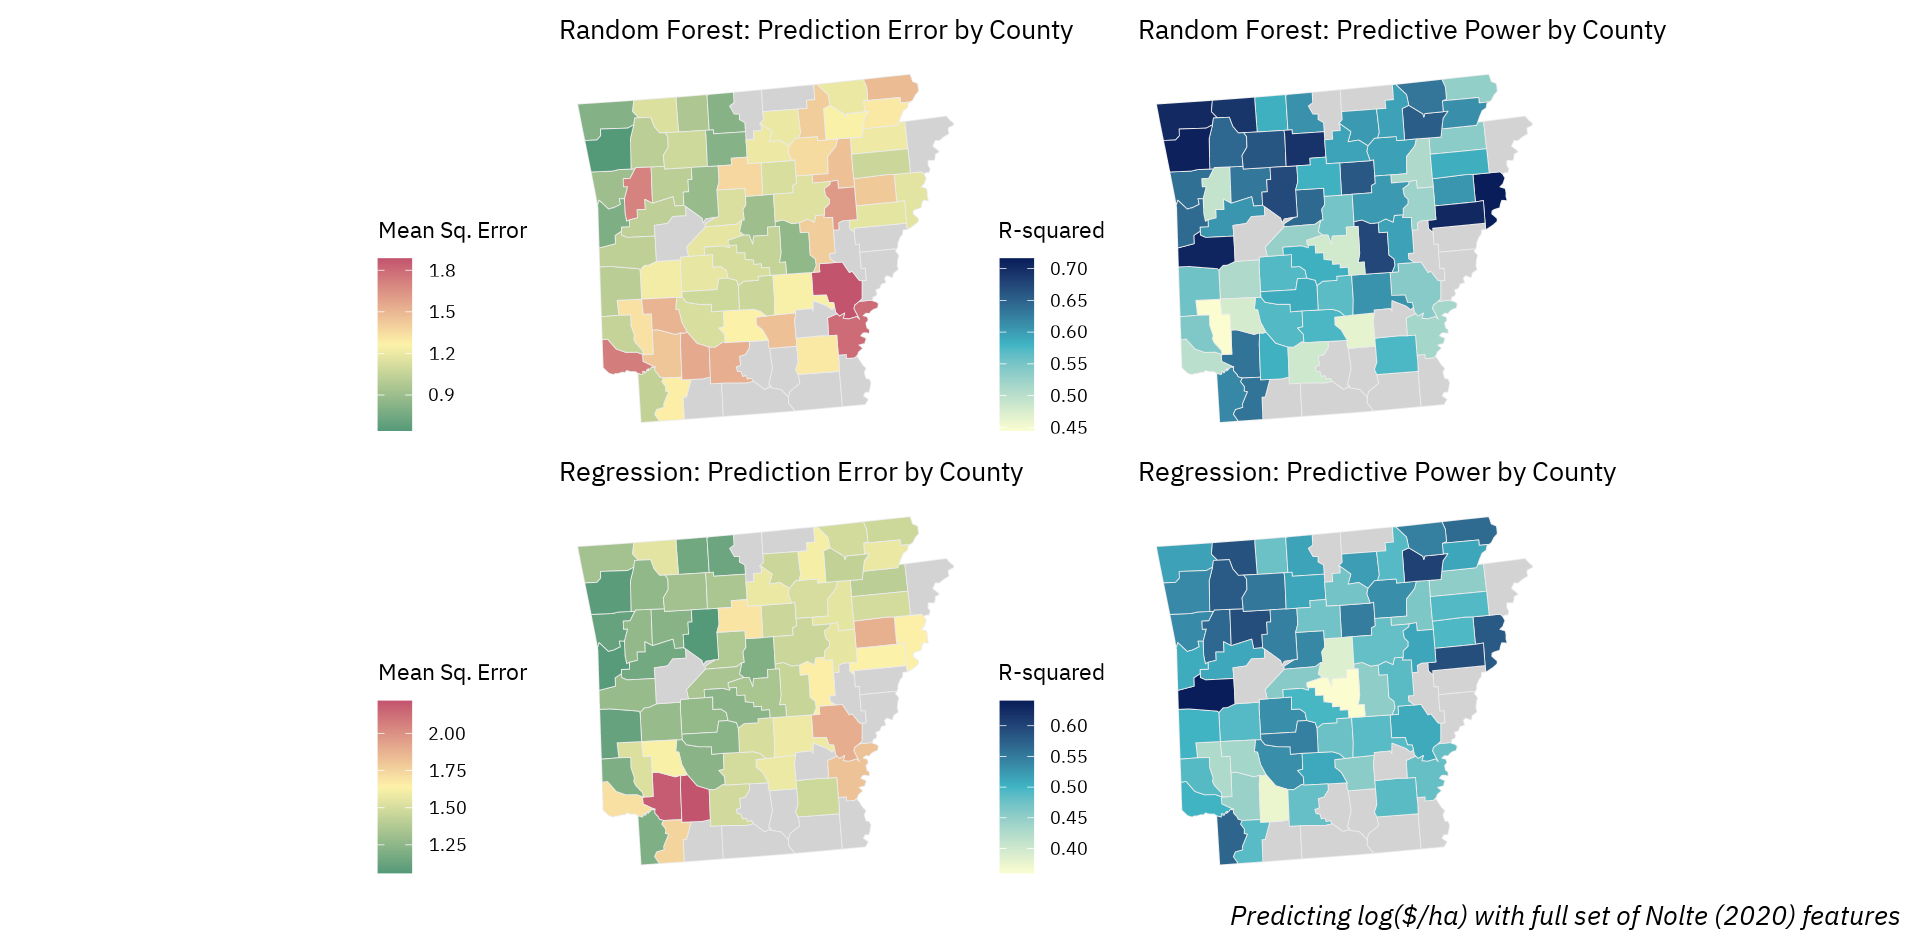
\includegraphics[width=6in]{eda_images/rf_reg_compare.png}
    \caption{Model Performance: Regression vs. Random Forest}
    \label{fig:model_compare}
\end{figure}

\newpage

\section{Discussion}

DISCUSSION

\newpage

\section{Conclusion}

CONCLUSION

\newpage

\section{Appendix}

\begin{itemize}
    \item Alternate Specifications
    \item Multi-parcel sale aggregation methods
\end{itemize}


\newpage


\printbibliography

\end{document}


